\documentclass[12pt]{article}

\usepackage{expex}
\usepackage[T1]{fontenc}
\usepackage[main=english,polish,spanish]{babel}
\usepackage{csquotes}       % For proper quotation formatting \enquote{}
\usepackage{hyperref}
\hypersetup{
    colorlinks=true,
    linkcolor=black,
    urlcolor=black,
    citecolor=black
}
\usepackage[style=apa, backend=biber, language=english]{biblatex} % APA 7th edition references

\usepackage{geometry} % 1-inch margins
\geometry{a4paper, margin=1in}
\usepackage{times} % Times New Roman font
\usepackage{setspace} % For double spacing
\usepackage{fancyhdr} % For headers and footers
\usepackage{titlesec} % For section numbering
\usepackage{booktabs} % For professional-looking tables
\usepackage{bookmark}
\usepackage{float}
\usepackage{graphicx}
\graphicspath{ {./figures/} }
\usepackage{caption}
\captionsetup[table]{font=footnotesize, labelsep= period, labelfont=bf, width=0.8\textwidth}
\captionsetup[figure]{font=footnotesize, labelsep= period, labelfont=bf, width=0.8\textwidth} 
% Options: tiny, scriptsize, footnotesize, small, normalsize, large, Large, etc.
\usepackage{subcaption}
\usepackage{tabularx}
\newcommand{\ts}[1]{\textsuperscript{#1}}
\newcommand{\ita}[1]{\textit{#1}}
\addbibresource{TFM.bib} % Reference file

% Set double spacing
\doublespacing

% Indent paragraphs by 0.5 inch
\setlength{\parindent}{0.5in}

% Page numbering setup
\pagestyle{fancy}
\fancyhf{}
\rfoot{\thepage} % Page number in the bottom-right corner
\renewcommand{\headrulewidth}{0pt} % Remove the header rule

% Section formatting
\titleformat{\section}[block]{\normalfont\Large\bfseries}{\thesection.}{0.5em}{}

\begin{document}
\pagenumbering{roman}
\section*{Abstract}
% This project investigates to what extent morphological inflection can be automatically distinguished from derivation based solely on word forms. The debate on inflection and derivation remains highly contentious in linguistic literature, with some viewing them as fundamentally similar or existing on a gradient, while others argue for a clear distinction. Despite extensive theoretical discussions, empirical evidence remains limited. One proposed distinction is semantic regularity: inflection is expected to be stable in its syntactic and semantic effects across lexemes (e.g., cinema is to cinemas as cat is to cats), whereas derivation is less so (e.g., delegation is not to delegate as election is to elect). However, this criterion has yet to be systematically tested large scale cross-linguistically. 
% Building on previous work (e.g., \textcite{bonami2018InflectionVsDerivation}; \textcite{rosa2019AttemptingSeparateInflection}), this project uses distributional semantics and word embeddings to assess semantic regularity as a potential proxy for differentiating inflection and derivation. It focuses on two morphologically rich languages, Spanish and Polish. Additionally, the project examines differences in semantic regularity also among various types of inflection, such as case, number, gender, and person.

\section*{Keywords}
morphology, inflection, derivation, distributional semantics, aspect in Polish

\newpage
\tableofcontents
\newpage

\pagenumbering{arabic}

\newpage
\section{Introduction}

Usually, a distinction between inflectional and derivational morphology is drawn. When we talk about inflection we are talking about the formation of grammatical words, also called word-forms, of a lexeme. A lexeme is an abstract word that acts as the representative of the meaning that all its word-forms relate to, so \textsc{bóbr} in the case of \autoref{tab:bobr} is the lexeme, and all the words that appear inside the different cells are its grammatical words. Verbs are also often used as examples of inflection, which change depending on the tense, aspect and mood. In \autoref{tab:conjugation} we can see the Spanish verb lexeme \textsc{comer} conjugated in three different tenses of the indicative mood. Generally, number, case, gender, person, tense, aspect and mood are expressed through inflectional processes \parencite{haspelmath2013UnderstandingMorphology,aronoff2011WhatMorphology}.

\begin{table}[htbp]
    \centering
    \footnotesize
    \renewcommand{\arraystretch}{1.2} % Adjust row height
    \begin{tabular}{lll} 
        \toprule
        & \textbf{Singular} & \textbf{Plural} \\ 
        \midrule
        \textbf{Nominative}   & bóbr   & bobry \\
        \textbf{Genitive}     & bobra  & bobrów \\
        \textbf{Dative}       & bobrowi & bobrom \\
        \textbf{Accusative}    & bobra  & bobry \\
        \textbf{Instrumental} & bobrem & bobrami \\
        \textbf{Locative}     & bobrze & bobrach \\
        \textbf{Vocative}     & bobrze & bobry \\
        \bottomrule
    \end{tabular}
    \caption{Declension of the Polish noun \textit{bóbr} `beaver'}
    \label{tab:bobr}
\end{table}



\begin{table}[htbp]
    \centering
    \footnotesize
    \renewcommand{\arraystretch}{1.2} % Adjust row height
    \begin{tabular}{llll} 
        \toprule
        & \textbf{Preterite} & \textbf{Present} & \textbf{Future} \\ 
        \midrule
       \textbf{\textsc{1sg}}  & comí   & como   & comeré \\
       \textbf{\textsc{2sg}}  & comiste   & comes  & comerás \\
       \textbf{\textsc{3sg}}  & comió      & come & comerá \\
       \textbf{\textsc{1pl}}  & comimos    & comemos  & comeremos \\
       \textbf{\textsc{2pl}}  & comisteis  & coméis & comeréis \\
       \textbf{\textsc{3pl}}  & comieron     & comen & comerán \\
     \bottomrule
    \end{tabular}
    \caption{Conjugation of the Spanish verb \textit{comer} `eat'.}
    \label{tab:conjugation}
\end{table}

\noindent
In the case of derivational morphology, it is involved in the creation of new lexemes, for instance through the use of the suffix \ita{-dor} or \ita{-ero} in Spanish in nouns such as \ita{abridor} `opener' from \ita{abrir} `open', \ita{casero} `landlord' from \ita{casa} `house'; or the suffix \ita{-ość} in Polish nouns like \ita{czystość} `cleanliness' from \ita{czysty} `clean'. When creating a new lexeme, the class (whether it is a noun, verb, adjective or adverb) may change, like in the previous examples of the deverbal noun \ita{abridor} `opener' and deadjectival noun \ita{czystość} `cleanliness' \parencite{haspelmath2013UnderstandingMorphology,booij2012GrammarWordsIntroduction}.

In order to draw a sharper boundary between both morphological processes authors propose many different criteria. 
For instance, it is said that inflection is relevant to the syntax but derivation is not. This means that what determines which form of a lexeme is used in a given position in a sentence is the relationship to the words around it \parencite{booij2012GrammarWordsIntroduction,aronoff2011WhatMorphology}. Still, inflection sometimes does not seem as relevant. Tense and aspect are rarely assigned by the syntax, so, following this criterion, they could be excluded from inflection \parencite{haspelmath2013UnderstandingMorphology}.
Another criterion, a relevant one regarding this thesis, is that in inflection the part of speech or category of the base does not change, while it may change in derivation \parencite{haspelmath2013UnderstandingMorphology} like it was shown before. However, there are some cases in which inflection is involved in a change of category like in gerunds or participles, which have properties of other parts of speech \parencite{booij2012GrammarWordsIntroduction}. 
The last relevant criterion is the semantic regularity criterion. It states that derivation expresses a new meaning but inflection does not change the lexical meaning \parencite{haspelmath2013UnderstandingMorphology} or, as put by \textcite{stump2017Inflection}, inflectional processes are semantically more regular than derivational processes. While it is true that a related noun and adjective like \ita{czystość} `cleanliness' and \ita{czysty} `clean' are also related in meaning, this relation is not like that of a verb and a conjugated form, like \ita{comer} `eat' and \ita{comiste} `you ate' \parencite{aronoff2011WhatMorphology}. In fact, \textcite{haspelmath2013UnderstandingMorphology} argue examples like the first one fall in between inflection and derivation.

Like we have seen, the distinction between these two processes is not without debate. For this reason, there have been authors that have challenged this sharp boundary view directly posing that we should not make a distinction between them \parencite{haspelmath2024InflectionDerivationTraditional} or that there is at best a continuum or gradient in which inflection and derivation stand on opposite sides \parencite{bybee1985MorphologyStudyRelation, stekauer2015DelimitationDerivationInflection}. \textcite{haspelmath2013UnderstandingMorphology} argue that if all criteria are given the same importance then a continuum is the best explanation, since a sharp boundary between both processes cannot be drawn. 
% \textcite{booij2006InflectionDerivation} also draws a distinction between two different inflectional processes, inherent (not required by syntax, but a semantic choice like the use of a plural form, infinitives, participles, tense, aspect and mood) and contextual (required by syntax, such as verb-subject agreement or a case choice in nouns). The author argues that inherent inflection is halfway between derivation and contextual inflection, since inherent inflection also may change the part of speech of a word.

% \subsection{Distributional semantics} \label{distributional-semantics}

In this thesis, in order to shed light on the inflection-derivation debate we explore the semantic regularity criterion using distributional semantics, a computational method to represent the meaning of words, based on the distributional hypothesis. This hypothesis essentially states that similar words appear in similar contexts, hence its distribution reflects its meaning. By examining the words around a given word, we can explore the relationships between them \parencite{boleda2020DistributionalSemanticsLinguistic}.
Distributional semantics represents the meaning of words as vectors, i.e. points in a multidimensional space, so similar words will also have similar a vector thus occupying a similar region in that space. In the semantic space created by a distributional semantics model we can see the relation between specific words looking at the geometric relations of their vectors, using either Euclidean distance (the length of the straight line between them) or, more commonly, cosine similarity (the cosine of the angle between the vectors). The higher the cosine similarity, the closer the vectors are to each other, meaning a higher semantic similarity \parencite{boleda2020DistributionalSemanticsLinguistic,chandrasekaran2021EvolutionSemanticSimilarity}. 
If we assume that derived lexemes stray further from the meaning of the base than inflected ones, while in inflection the core meaning stays the same, then distributional semantics is a great way to explore this criterion. Consequently, inflectional processes should maintain more similarity in meaning than derivational processes in a vector space, i.e. the relation between words related by an inflectional process should be closer than the relation between words related by a derivational process. % To test this, the similarity between a lemma (pivot) and its inflected forms was measured for each of the forms. The similarity between a lemma and a derived form was also measured and then averaged and compared to the inflectional mean.

There are three recent studies that have advanced our understanding of how distributional semantics can contribute to the inflection-derivation debate. \textcite{bonami2018InflectionVsDerivation} conduct a distributional study in order to assess if inflection is semantically more regular than derivation. They conclude that a categorical boundary between inflection and derivation cannot be found, although inflectional relations are more semantically stable on average. For their study they use a French lexicon and their own French embeddings model, a continuous bag of words (CBOW) model with negative sampling, subsampling, a window size of 5 and a vector size of 400, they construct a triplets dataset consisting of a pivot, an inflectional comparandum and a derivational comparandum based on different frequency measures. In their experiment, they measure shifts in meaning, measuring vector offset variance using Euclidean distance between the inflectional comparandum and the derivational comparandum. The authors clarify that using cosine similarity gives similar results on their data. \textcite{rosa2019AttemptingSeparateInflection} use a FastText Czech model (although they puposefully ignore words that do not appear in the model) to automatically separate inflection and derivation using a different criterion, the lexical meaning change criterion. They aim to determine if two morphologically related words belong to the same inflectional paradigm or are linked by derivation. Using a Czech database of word formation relations they measure string similarity (Jaro-Winkler edit distance) and cosine similarity. They broadly find that inflectional forms are more similar to each other than derivational forms. Taking into account only the measure of cosine similarity, they find it separates inflection and derivation adequately, although negation (using the prefix \ita{-ne}) and grade inflection possess a high cosine similarity, closer to derivation, than widely accepted inflectional processes like case marking or number. Combining both measures, derivation continues to be separated from inflection, although negation shows lower similarity than derivation. Exploring derivations in detail, they find high cosine similarity in aspectual morphology regarding the change of a perfective verb to its imperfective counterpart, a traditionally considered (in Czech) category-preserving derivational process, i.e. a process that does not change the category or part of speech. In some category-changing derivation, like between \textsc{n} and \textsc{v} they find lower cosine similarity but higher in \textsc{adj} to \textsc{adv} or \textsc{n} to \textsc{poss adj}. Finally, \textcite{haley2024CorpusbasedMeasuresDiscriminate} conducted a study trying to classify constructions into inflection or derivation in 26 languages. The authors computed four measures, two based on the orthographic form and two on the distributional characteristics, to predict whether a given construction is inflectional or derivational using UniMorph data and two types of machine learning models. Like the previous study, they used FastText models for all of the languages. What they find is that their best model can correctly predict the morphological process most of the time (89\% +-1) but many constructions lie between both categories. Their results indicate that there is no strict boundary between inflection and derivation, but that they belong to a gradient

One factor these studies do not explore in detail is the change of category in derivation, it is only shortly mentioned in \textcite{rosa2019AttemptingSeparateInflection}. As it has been pointed out before, derivation may or may not change the category of the lexeme it creates. This is a key element that it is worth exploring, specially due to the fact that it is one of the mainly referenced criteria to distinguish between inflection and derivation. For this reason, this thesis aims to explore the difference between category-preserving and category-changing derivational processes using distributional semantics models.

Additionally, we are interested in exploring a linguistic question between inflectional processes and category-preserving derivational processes, thus the consideration to examine this in more detail. Similarly as it was pointed out in \textcite{rosa2019AttemptingSeparateInflection} regarding Czech, some processes involving aspect in Polish are not agreed upon. Specifically, a way of forming perfective verbs from imperfectives and a way of forming imperfective verbs from derived perfective verbs. Verbs in Polish have traditionally been described as having a counterpart in the opposite aspect, i.e. an imperfective verb such as \ita{pisać} (write.\textsc{ipfv}) has a perfective pair, in this case \ita{napisać} (write.\textsc{pfv}). These perfective pairs are formed by so-called empty prefixes, prefixes that only change the aspect of the verb and do not add any meaning, hence this process is usually considered inflectional. In some cases, aspectual pairs are not created with an empty prefix, but through suffixation from a perfective verb, like in \ita{kupić} (buy.\textsc{pfv}) -- \ita{kupować} (buy.\textsc{ipfv}). Deriving new verbs from imperfective ones is done through prefixation and the resulting ones are generally perfective, e.g. \ita{podpisać} (sign.\textsc{pfv}) derived from the previous verb \ita{pisać} (write.\textsc{ipfv}). Since the resulting derived verb is perfective, it needs an imperfective counterpart, in which case it is commonly obtained through suffixation, e.g. \ita{podpisywać} (sign.\textsc{ipfv}). These imperfective verbs are called secondary imperfectives, and this process is also generally considered an inflectional one. In a nutshell, the points of contention are many. Some authors consider that empty prefixes do add some change in meaning, therefore this process should be considered derivational, while others maintain there is no change. The ones that reject empty prefixes only consider suffixed imperfective forms as true aspectual pairs, but others argue that there is also a change in meaning in secondary imperfectivization, excluding them from the true aspectual pairs. In this case the only true aspectual pairs would be non-prefixed perfective verbs and their suffixed imperfective counterpart, i.e \ita{kupić} (buy.\textsc{pfv}) -- \ita{kupować} (buy.\textsc{ipfv}). This is described and investigated in more detail in the second study of this thesis (see \autoref{polishaspect}). 

In this fashion, the objectives of this thesis are two-fold: exploring the inflection-derivation debate emphasizing category-preserving and caregory-changing derivation by means of distributional semantics, and, using the same methods, trying to shed light on a theoretical debate regarding aspectual morphology in Polish.

% - You need to state what the gaps on these studies. And you need to already point out that they do not make explicit distinctions between category-preserving and category-changing derivational processes. And given that this is one of the main descriptions of the derivation/inflection divide, it is word to look into that with more granularity. And see if what differences remain after taking those distinctions into account.

% After you have introduced all this, it should now be clear: the background, the two goals of the study (category-preserving vs categoru-chaning continuum, and using this to shed light on current linguistic debates in Polish aspect morphology), and their motivation.

\section{First study} \label{first}
\subsection{Methodology} \label{methodology1}

This study explores the distinction between inflection and derivation in Polish and Spanish using two static word embedding models: Word2Vec \parencite{mikolov2013EfficientEstimationWord} and FastText \parencite{bojanowski2017EnrichingWordVectors}. The main difference between both is that Word2Vec operates on a word level and FastText on a subword level. This means a Word2Vec model has vector representations for whole words but FastText for subwords. In case the models encounter words that were missing from its training data, only a FastText model can compute word representations for such words \parencite{bojanowski2017EnrichingWordVectors}. Specifically, the chosen Spanish Word2Vec embeddings model was trained on the Spanish Billion Words (SBW)\footnote{\url{https://crscardellino.net/SBWCE/}} corpus \parencite{cardellino2016SpanishBillionWord}. For Polish, the IPIPAN Word2Vec embeddings model \textit{nkjp+wiki-forms-all-300-skipg-ns}\footnote{\url{https://dsmodels.nlp.ipipan.waw.pl/}} was used. This one was specifically chosen because it resembles the SBW model in vector dimension and training method. It was trained with the \texttt{gensim} library using the skip-gram algorithm with negative sampling on the National Corpus of Polish (NKJP)\footnote{\url{https://nkjp.pl/}} and Wikipedia, includes all parts of speech and word forms, and produces 300-dimensional vectors. Regarding the FastText embeddings, the ones used are the newest version available in the FastText\footnote{\url{https://fasttext.cc/}} site for both languages \parencite{grave2018LearningWordVectors}. 

The data that was used was taken from UniMorph (Universal Morphology), a resource that provides annotated morphological inflection tables for hundreds of languages \parencite{batsuren2022UniMorph40Universal}. It offers a standardized schema for encoding morphological features such as tense, mood, number, person, case, and gender. The project compiles and normalizes inflectional paradigms extracted primarily from Wiktionary, producing tabular datasets that list all known inflected forms of a lemma alongside their corresponding morphological features (\autoref{tbl:unimorph-inf}). With the release of UniMorph 4.0 they included derivational information and an annotation schema to represent derivational processes (\autoref{tbl:unimorph-der}).

\begin{table}[htbp]
    \footnotesize
    \centering
    \begin{tabular}{p{3cm}p{3.5cm}p{4.5cm}}
        \toprule
        universalizar & universalizarás &  V;IND;FUT;2;SG;INFM \\
        desguanguañar & desguanguañamos & V;IND;PRS;1;PL \\
        desencorvar  &    desencorvo    &   V;IND;PRS;1;SG \\
        nutrir    &      nutrían  &  V;IND;PST;IPFV;3;PL \\
        innovar    &     innovaré    &   V;IND;FUT;1;SG \\
    \end{tabular}
        \begin{tabular}{p{3cm}p{3.5cm}p{4.5cm}}
        \midrule
        zakazać        &  zakazał   &    V;PST;3;SG;MASC \\
        ścignąć         &  ścigną &           V;FUT;3;PL \\
        zadzwonić &  zadzwoniliście &  V;PST;2;PL;MASC;HUM \\
        umówić się        &  umówiło &      V;PST;3;SG;NEUT \\
        zaniechać &  zaniechałyście &           V;PST;2;PL \\
        \bottomrule
    \end{tabular}
    \caption{Sample from the Spanish (top) and Polish (bottom) UniMorph inflectional dataset.}
    \label{tbl:unimorph-inf}
\end{table}

\begin{table}[htbp]
    \footnotesize
    \centering
    \begin{tabular}{p{2.5cm}p{3cm}p{2.5cm}p{2.5cm}}
        \toprule
        lluvia   &      lluvioso   &  N:ADJ &   -oso \\
        transformar &  transformación &     V:N &   -ción\\
        comparable & comparablemente & ADJ:ADV &  -mente\\
        pirita &     calcopirita &     N:N &  calco-\\
        desintoxicar &  desintoxicante &   V:ADJ &   -ante\\
    \end{tabular}
    \begin{tabular}{p{2.5cm}p{3cm}p{2.5cm}p{2.5cm}}
        \midrule
        namierzyć  &     namierzenie     &  V:N &   -enie \\ 
        żywczanin  &       żywczanka     &  N:N &     -ka\\ 
        wykrwawić  &      wykrwawiać     &  V:V &     -ać\\ 
        hejnał     &   hejnałowy   &  N:ADJ   &   -owy\\ 
        zadrzeć    &     zadarcie     &  V:N   &  -cie\\ 
        \bottomrule
    \end{tabular}
    \caption{Sample from the Spanish (top) and Polish (bottom) UniMorph derivational dataset.}
    \label{tbl:unimorph-der}
\end{table}

In order to conduct the analysis two separate datasets were built for each language, one for inflection and another one for derivation, filtering the necessary data from UniMorph and cleaning it afterwards. For the inflectional morphology analysis, a lemma-inflection-category dataframe was constructed. The data was filtered to include the following verb tenses in Spanish: Present Indicative (UniMorph tag: \textsc{v;ind;prs}), Past Imperfect (UniMorph tag: \textsc{v;ind;pst;ipfv}) and Future Indicative (UniMorph tag: \textsc{v;ind;fut}). A second filter was applied on the resulting data to remove \textit{vos} and \textit{usted} forms. \textit{Voseo} forms do not have a high occurrence and \textit{usted} forms are essentially duplicated forms since they are the same as 3rd person singular forms. In Polish, the filtering included the same verb tenses: Present (UniMorph tag: \textsc{v;prs}), Past (UniMorph tag: \textsc{v;pst}) and Future (UniMorph tag: \textsc{v;fut}).

For the derivational morphology analysis, the label \textsc{u} (unknown) in UniMorph was either fixed or removed in the final dataframe. In the Spanish data, there were 20 rows that contained a derivational process that results in \textsc{u} (i.e. \textsc{x:u}, where the lemma is to the left of the colon and the derived word is on the right) and 107 in Polish. On the other hand, there were even more rows in which the lemma was tagged \textsc{u} (\textsc{u:x}), 36 in Spanish and 253 in Polish.
In order to clean the Spanish derivations dataset a new category according to the affix of the row was assigned to the lemma position. All the lemmas that end in \textit{-ero}, \textit{-ez}, \textit{-ismo}, \textit{-í} and \textit{-illa} were changed from \textsc{U} (\textsc{u:x}) to \textsc{n} (\textsc{n:x}), since all these are noun affixes. The category was also changed to \textsc{v:x} in those that contain the affixes \textit{-ar} and \textit{-ear}. As a result 6 rows were left over and eliminated from the final dataframe because they simply contained mistakes. The rows which were tagged \textsc{u} in the derivation position (\textsc{x:u}) were dropped because they contained numerals and words that are not nouns, adjectives, adverbs or verbs. The latter were simply dropped, and since numerals could be tagged as either \textsc{n} or \textsc{adj}, they could also be dropped. In total, only 36 rows were discarded, which will not have major influence on the results.

Regarding the fixes in the Polish derivational data, some rows incorrectly labelled \textsc{u} in the derivation position (\textsc{x:u}) were fixed by looking at the affix column. The rows containing affixes \textit{-any}, \textit{-ony}, \textit{-ty}, \textit{-y}, or \textit{-ący}, \textit{-ęty} were changed to \textsc{x:adj} as these are endings taken by participles. Some formatting issues were also fixed, like rows in the lemma position which contained both the lemma and the derived form (e.g. \textit{mylićpomylić pomylić}). Some rows that contained verbs in both columns but were not correctly labeled in the derivation form (\textsc{v:u}) were fixed as well. Three specific rows incorrectly labeled \textsc{u:u} were changed to \textsc{adj:adj} since they contained adjectives. The left over rows could be removed as well as they did not contain any nouns, adjectives, adverbs or verbs.
Tackling the lemma position, there were many rows (163) that contained infinitives in both columns but were incorrectly labelled \textsc{u:v} instead of \textsc{v:v}. Since infinitives in Polish end in \textit{-ć} or \textit{-c} this was a straightforward fix. After that, there were few rows (21) with issues. Just like in previous instances, these rows contained words that are not nouns, adjectives, adverbs or verbs and they were dropped as a result. In the end, all four dataframes (inflection and derivation in Spanish and Polish) do not contain any row labeled with \textsc{u} anymore.

After the data processing was done, a Python script was written and used on the four dataframes (inflection and derivation in Spanish and Polish). In this script, the vector of the lemma and the vector of the second item (either the inflected form or the derived word) were obtained row by row. Afterwards, the cosine similarity of the two vectors was calculated using the \texttt{cosine} function of the \texttt{scipy} library and it was added to the dataframe. This data was exported afterwards for future an analysis in R \parencite{rlanguage}. This automatic process was run using both word embedding models and both languages in inflection and derivation.

\subsection{Results} \label{results1}

We fit two Bayesian Beta regression hierarchical models to assess differences in cosine similarity across three types of affixation: category-changing derivation, category-preserving derivation, and inflection. In both models, affixation type was included as the only fixed effect. As random effects, we included intercepts for model (word2vec and FastText), language (Polish and Spanish), and their interaction. We set the same Student-t prior ( df = 5 , $\mu$ = 0 , $\sigma$ = 3) on all fixed effects, including the intercept. For the random effects, we used a half Student-t prior ( df = 3 , $\mu$ = 0 , $\sigma$ = 2.5). The precision parameter $\varphi$ was assigned a weakly informative Gamma prior ($\alpha$ = 0.01 , $\beta$ = 0.01).

In the first model, the fixed effect is Helmert contrast-coded. We compare the mean cosine similarity of category-preserving derivation (type1) to category-changing derivation, and the mean cosine similarity of inflection (type2) to the average of the previous two. In the second model, the fixed effect is treatment-coded, with the reference level set to category-preserving derivation. We thus compare category-changing derivation and inflection separately to category-preserving derivation.

The Beta model with Helmert coding reveals a strong effect of affixation type on cosine similarity. Specifically, category-preserving derivation shows higher similarity than category-changing derivation (estimate = 0.235, 90\% CI [0.136, 0.335], posterior probability > 0 = 1.000). There is also moderate evidence that inflectional forms are more similar than the average of the two derivational types (estimate = 0.041, 90\% CI [0.000, 0.083], posterior probability > 0 = 0.949).

In the Beta model with treatment coding (reference level: category-preserving derivation), cosine similarity varied across affixation types. Category-changing derivation showed substantially lower similarity than category-preserving derivation (estimate = -.471, 90\% CI [-0.672, -0.269], posterior probability < 0 = 1.000). In contrast, there was little evidence for a difference between inflection and category-preserving derivation (estimate = -0.113, 90\% CI [-0.298, 0.074], posterior probability < 0 = 0.838). The intercept, representing the mean similarity for category-preserving derivation, was estimated at 0.157 (90\% CI [-0.934, 1.298]), with low certainty that it differed from zero (posterior probability > 0 = 0.639).

% CLEAN DATA FIGURE
\begin{figure}[htbp]
\centering
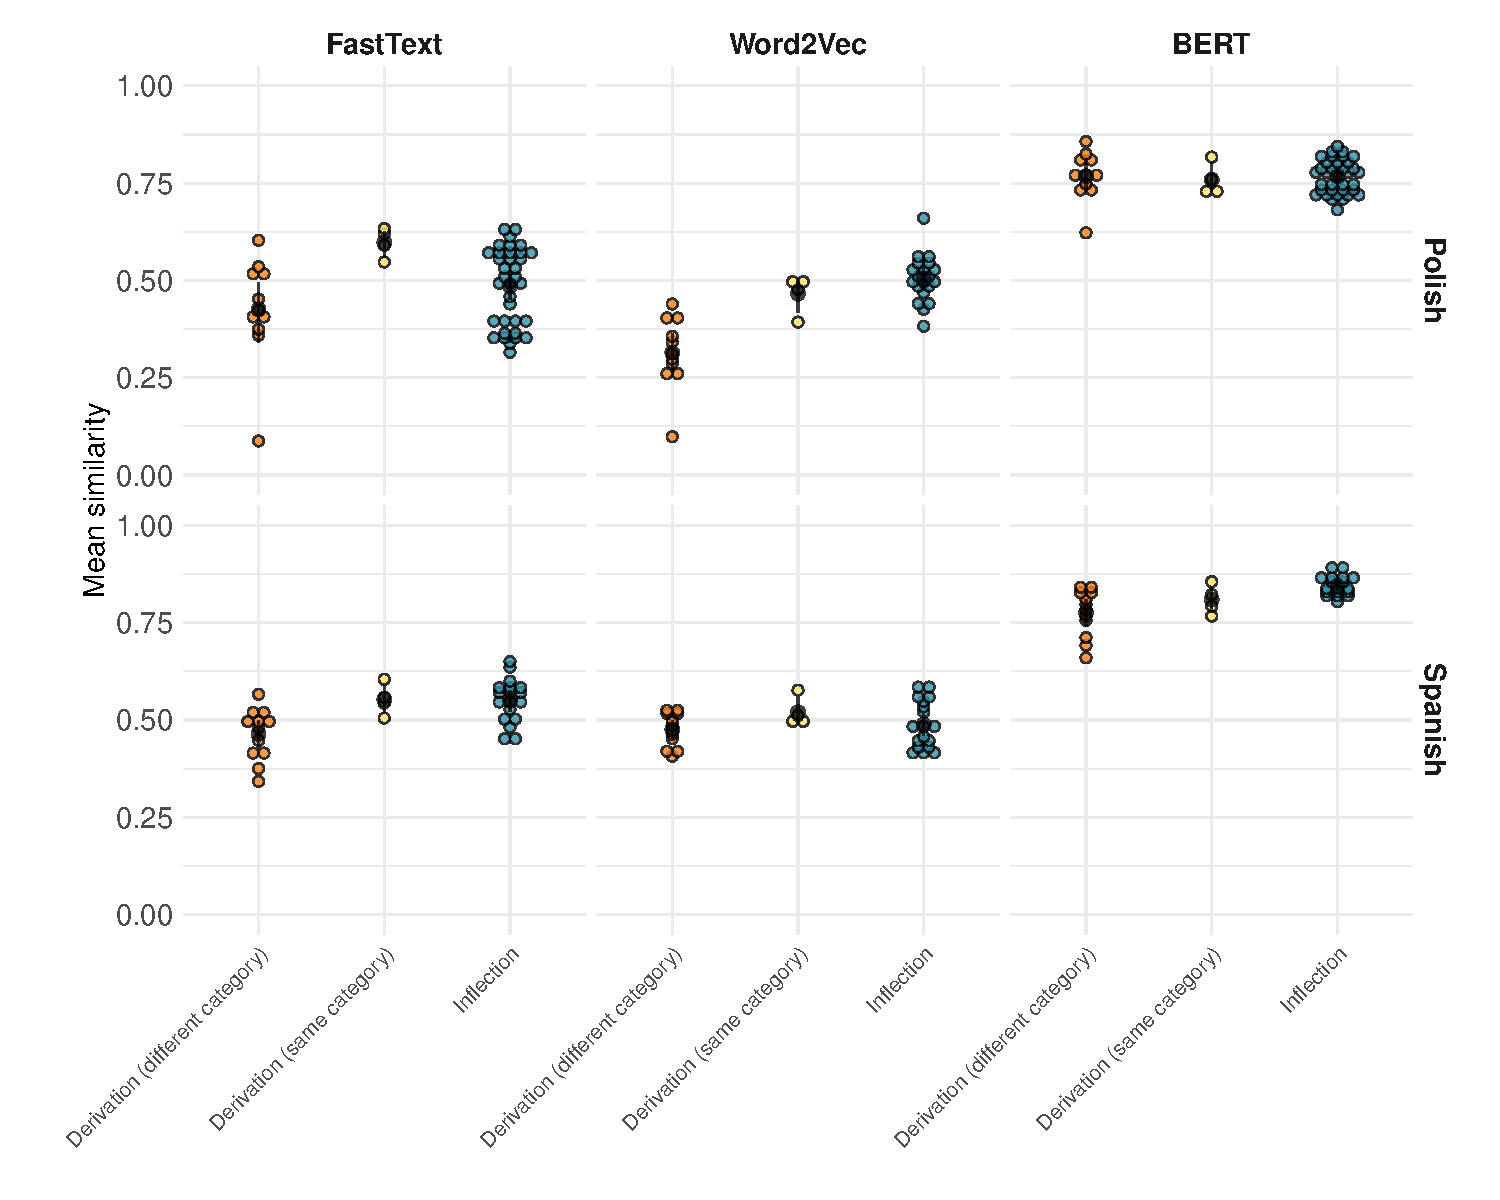
\includegraphics{fig-clean.pdf}
\caption{Similarity between lemma and inflectional or derivational element by model and language. Each coloured dot represents a category in derivation and a different conjugation form (number, person and tense) in inflection. The black dot represents the mean similarity of the whole morphological process, with the standard deviation around it.}
\label{fig:clean-data}
\end{figure}

% CLEAN DATA TABLE
\begin{table}[h!]
\centering
\label{tbl:mean-similarity}
\begin{minipage}[t]{0.48\textwidth}
\footnotesize
\centering
\subcaption*{Inflection}
\begin{tabular}{llc}
\toprule
\textbf{Model} & \textbf{Language} & \textbf{Mean similarity} \\
\midrule
\textbf{FastText}  & Spanish & 0.55 \\
                   & Polish  & 0.48 \\
\textbf{Word2Vec}  & Spanish & 0.53 \\
                   & Polish  & 0.51 \\
\bottomrule
\end{tabular}
\end{minipage}
\hfill
\begin{minipage}[t]{0.48\textwidth}
\footnotesize
\centering
\subcaption*{Derivation}
\begin{tabular}{llc}
\toprule
\textbf{Model} & \textbf{Language} & \textbf{Mean similarity} \\
\midrule
\textbf{FastText}  & Spanish & 0.51 \\
                   & Polish  & 0.54 \\
\textbf{Word2Vec}  & Spanish & 0.50 \\
                   & Polish  & 0.40 \\
\bottomrule
\end{tabular}
\end{minipage}
\caption{Mean similarity between lemma and inflectional or derivational element by model and language.}
\end{table}

In order to evaluate the effectiveness of the methods and provide a point of comparison, the mean similarity of the target pairs in the data was compared to a random baseline. This baseline filtered the data separately, inflections by tense (present, past or future) and derivations by category (\textsc{n:adj}, \textsc{v:n}\dots). After filtering, each individual part was shuffled 100 times while extracting the mean similarity of every row and the average of all rows. In other words, the mean similarity was extracted 100 times by type of morphological process (inflection or derivation), tense/category, model and language. The distribution is shown in \autoref{fig:baseline}.

% BASELINE FIGURE
\begin{figure}[!htbp]
\centering
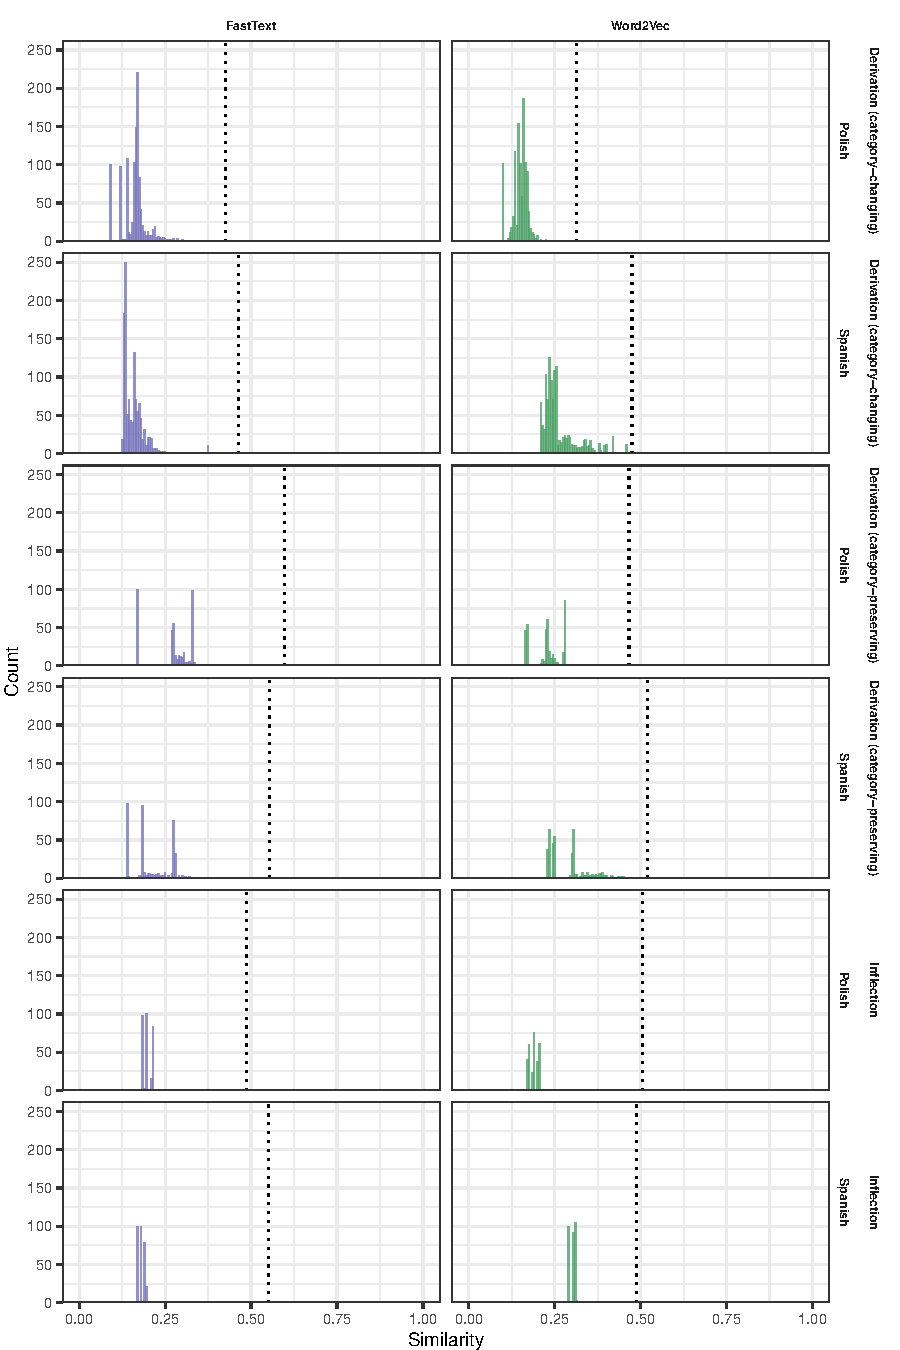
\includegraphics[height=20cm]{fig-baseline-faceted.pdf}
\caption{Distribution of the random baseline. Each datapoint represents an instance of the mean similarity of the type of morphological process, tense/category, model and language. The dotted line represents the mean similarity value by category/tense on the data.}
\label{fig:baseline}
\end{figure}

\subsection{Discussion} \label{discussion1}

% talk about the results and all, shortcomings?

We find evidence for a difference between inflection and derivation when category-preserving and category-changing derivation are not distinguished, and inflection is compared to their average (Helmert-coded model). However, when using treatment coding and directly comparing inflection to category-preserving derivation, no strong difference emerges. Across both models, there is strong evidence that category-preserving derivation differs from category-changing derivation, with the latter showing substantially lower cosine similarity.

\newpage
\section{Second study} \label{second}

\subsection{The morphology of aspect in Polish} \label{polishaspect}

The traditional view in Polish is that verbs come in pairs, one being imperfective and the other being perfective, which are generally distinguished by prefixes or suffixes \parencite{nagorko2010PodrecznaGramatykaJezyka}. Take for instance the verb \textit{pisać} (write.\textsc{ipfv}). In order to fully express what you would using one verb in English, you also need to know its aspectual pair \textit{napisać} (write.\textsc{pfv}). The prefix \textit{na-} is what is called an empty prefix, that is a prefix that changes the aspect of the verb and does not alter its meaning. However, the existence of empty prefixes and what aspectual pairs really are is a contentious topic that will be addressed later. In Polish, the perfective aspect refers to completed actions that result in changes in the state of affairs, while the imperfective refers to other types of actions: on-going, habitual, or complete but not causing a change in the state of affairs \parencite{swan2002GrammarContemporaryPolish}. The meaning behind the imperfective-perfective opposition also depends on the meaning of the verb itself, take for instance \textit{stukać} (knock.\textsc{ipfv}) -- \textit{stuknąć} (knock.\textsc{pfv}). In the perfective aspect, this verb implies just one knock, but in the imperfective it implies there were many knocks. Compare it to \textit{pisać} (write.\textsc{ipfv}) -- \textit{napisać} (write.\textsc{pfv}) where \textit{napisać} does not mean `write just once' but `write until the end, finish writing'. With other types of verbs such as \textit{rozumieć} (understand.\textsc{ipfv}) -- \textit{zrozumieć} (understand.\textsc{pfv}), the perfective form does not imply an ending to the understanding, but rather a beginning  \parencite{nagorko2010PodrecznaGramatykaJezyka}.
To form the perfective of an imperfective verb a prefix may be employed, like the previously mentioned \textit{pisać} (write.\textsc{ipfv}) -- \textit{napisać} (write.\textsc{pfv}). It can also be done with the semelfactive suffix \textit{-ną} (\textit{krzyczeć} (shout.\textsc{ipfv}) -- \textit{krzyknąć} (shout.\textsc{pfv})). On the contrary, to form the imperfective from a perfective verb a suffix or morphophonological modification is employed (\textit{kupić} (buy.\textsc{pfv}) -- \textit{kupować} (buy.\textsc{ipfv}); \textit{ocenić} (mark.\textsc{pfv}) -- \textit{oceniać} (mark.\textsc{ipfv})) \parencite{bloch-trojnar2015GrammaticalAspectLexical}. 
Prefixation can also generate more verbs with a different lexical meaning, all in the perfective aspect (generally), see \autoref{tab:derived-pisac}. A thing to note about perfective verbs is that they are defective, since they cannot be used to refer to the present only to the past and the future, while imperfective verbs have all three tenses. The imperfective future tense is formed using \textit{być} (be.\textsc{ipfv}) as an auxiliary in the future tense, while in perfective verbs it is formed synthetically \parencite{willim2006EventIndividuationCountability}.

 \begin{table}[h!]
    \centering
    \small
    \begin{tabular}{p{2.5cm}l}
        \toprule
        \textbf{Imperfective} & \textbf{Perfectives} \\ 
        \midrule
        \textit{pisać} `write' & \textit{dopisać} `add'  \\
         & \textit{popisać} `scribble' 	 \\
         & \textit{wpisać} `write in' 	 \\
         & \textit{podpisać} `sign' \\
         & \textit{zapisać} `fill' \\
         & \textit{prepisać} `copy' \\
         & \textit{opisać} `describe' \\
         & \textit{odpisać} `write back' \\
        \bottomrule
    \end{tabular}
    \caption{Examples of derived verbs of the verb \textit{pisać} (write.\textsc{ipfv}).}
    \label{tab:derived-pisac}
\end{table}


Many of the derived verbs relate to the meaning of \textit{pisać} (write.\textsc{ipfv}) in that the actions are also done in writing, \textit{dopisać} (add.\textsc{pfv}) is `adding while writing', przepisać (copy.\textsc{pfv}) is `copying while writing',  while some others do not, in \textit{opisać} (describe.\textsc{pfv}) the meaning is not limited to a writing context. 
After seeing these examples, one might come to the conclusion right away that the prefixes contain predictable meaning. This is partly true since these prefixes are also prepositions, so the meaning can be predictable at times, although it is often complicated. Take for instance \textit{za-}, which has 8 meanings assigned to it \parencite[Śmiech, 1986, as cited in][]{kita2017WybieramGramatykeDla}: \textit{grać} (play.\textsc{ipfv}) -- \textit{zagrać} (play.\textsc{pfv}); \textit{bić} (hit.\textsc{ipfv}) -- \textit{zabić} (kill.\textsc{pfv}); \textit{brać} (take.\textsc{ipfv}) -- \textit{zabrać} (earn.\textsc{pfv}); \textit{dać} (give.\textsc{ipfv}) -- \textit{zadać} (ask.\textsc{pfv}); \textit{trzymać} (hold.\textsc{ipfv}) -- \textit{zatrzymać} (stop.\textsc{pfv}) \parencite{perlin2005IleJestAspektow}. Another thing that is not predictable is which prefix is the one that functions as an empty prefix, so one must always know it by heart.

Regarding now suffixation and morphophonological modification, these are often associated with imperfectivizing perfective verbs. This generalization does not hold when it comes to the previously mentioned semelfactive suffix \textit{-ną}, which is used in the creation of perfective verbs, like it was pointed out in \textit{krzyczeć} (shout.\textsc{ipfv}) -- \textit{krzyknąć} (shout.\textsc{pfv}) or \textit{stukać} (knock.\textsc{ipfv}) -- \textit{stuknąć} (knock.\textsc{pfv}). Derived verbs, i.e. prefixed verbs that have a different lexical meaning, shown in \autoref{tab:derived-pisac}, can be further imperfectivized. These imperfective forms of derived perfective verbs are called secondary imperfectives and they can be formed either with the suffix \textit{-yw-/-i\textit{w}-}, alternating the thematic vowel or suffix, or with a stem alternation. We can see examples of some secondary imperfectives provided by \textcite{willim2006EventIndividuationCountability} in \autoref{tab:simpf}.

% change the name of the process: suffixation and morphophonological modification, stem alternation, affix alternation?...

 \begin{table}[h!]
    \centering
    \small
    \begin{tabular}{p{2.5cm}p{3cm}l}
        \toprule
        \textbf{Imperfective} & \textbf{Derived perfective} & \textbf{Secondary impf.} \\ 
        \midrule
        \textit{kupić} `buy' & \textit{przekupić} `bribe'	& \textit{przekupywać}  \\
        \textit{bić} `hit' & \textit{przebić} `pierce'	& \textit{przebijać} 	 \\
        \textit{służyć} `serve' & \textit{zasłużyć} `deserve'  & \textit{zasługiwać}	 \\
        \textit{brać} `take' & \textit{obrać}	`peel' & \textit{obierać}  \\
        \bottomrule
    \end{tabular}
    \caption{Examples of secondary imperfectives.}
    \label{tab:simpf}
\end{table}

% citar a laskowski en grzegorczykowa?
Under this simple overview, it seems prefixed forms are formed by derivational processes and suffixed forms by inflectional processes. Some authors (\textcite{grzegorczykowa1999Morfologia,wlodarczyk2006SemanticStructuresAspect,nagorko2010PodrecznaGramatykaJezyka,perlin2005IleJestAspektow} among others) support this dual view of aspect, with some caveats. One issue this analysis has is aspectual pairs formed by prefixation (\textit{pisać} (write.\textsc{ipfv}) -- \textit{napisać} (write.\textsc{pfv})), since the only difference between both is the aspect, while there is no difference in lexical meaning. Due to this, some of them, like \textcite{nagorko2010PodrecznaGramatykaJezyka}, say that the formation of aspectual pairs is an inflectional process, even those formed by prefixation, although others still place that specific type of aspectual pairs under derivation, like \textcite{grzegorczykowa1999Morfologia}, who argue that the choice of an empty prefix is lexically motivated since you cannot predict which one a given verb will take, thus they list both aspect forms under different lexemes. They also note that some verbs have more than one aspectual pair with an empty prefix, like \textit{brudzić} (soil.\textsc{ipfv}) -- \textit{zabrudzić} (soil.\textsc{pfv}) -- \textit{pobrudzić} (soil.\textsc{pfv}). \textcite{perlin2005IleJestAspektow} adds some more arguments to this, such as the change in meaning when adding a prefix is irregular and that the addition of it does not always change the aspect of the verb: \textit{pływać} (swim/sail.\textsc{ipfv}) -- \textit{wypływać} (flow out/surface.\textsc{ipfv}), \textit{chodzić} (go/walk.\textsc{ipfv}) -- \textit{dochodzić} (arrive.\textsc{ipfv}), \textit{wieszać} (hang.\textsc{ipfv}) -- \textit{rozwieszać} (hang clothes.\textsc{ipfv}). This author also points out that sometimes some prefixes change the aspect while some others do not, on the same verb: \textit{biegać} (run.\textsc{ipfv}) -- \textit{wybiegać} (run out.\textsc{ipfv}) but \textit{pobiegać} (run for a while.\textsc{pfv}). In a similar way, some other authors, like \textcite{wlodarczyk2006SemanticStructuresAspect} among others, reject the existence of empty prefixes since all verbal prefixes have some semantic weight. Given that the perfective may be expressed by many verbs derived from a single one (see all the derived perfectives in \autoref{tab:derived-pisac}), there is no true aspectual pair formed by empty prefixes since this type of pairs have a slightly different meaning, they argue, although \textcite{grzegorczykowa1999Morfologia}  do not go that far.

\textcite{wlodarczyk2006SemanticStructuresAspect} also consider only true aspectual pairs suffixed imperfective forms or morphophonologically altered forms, like \textit{przepisywać} (copy.\textsc{ipfv}) from \textit{przepisać} (copy.\textsc{pfv}) or \textit{zamawiać} (order.\textsc{ipfv}) from \textit{zamówić} (order.\textsc{pfv}). Contrary to this, \textcite{grzegorczykowa1999Morfologia} claim that imperfective forms of derived prefixed forms are not true aspectual pairs, since the meaning changes to iterative. Under their analysis, unprefixed pairs like \textit{kupić} (buy.\textsc{pfv}) -- \textit{kupować} (buy.\textsc{ipfv}) are true aspectual pairs formed by inflection and prefixed pairs like \textit{przepisać} (copy.\textsc{pfv}) -- \textit{przepisywać} (copy.\textsc{ipfv}) are formed by derivation and are not true aspectual pairs. On the other hand, \textcite{perlin2005IleJestAspektow} argues for an inflectional analysis of aspectual pairs, although he calls it the imperfective-perfective opposition and supports the existence of empty prefixes. The author lists six morphological processes involved in aspectual pairs: (1) suppletism, \textit{brać} (take.\textsc{ipfv}) -- \textit{wziąć} (take.\textsc{pfv}), \textit{widzieć} (see.\textsc{ipfv}) -- \ita{zobaczyć} (see.\textsc{pfv}); (2) prefixation, \ita{myć} (wash.\textsc{ipfv}) -- \ita{umyć} (wash.\textsc{pfv}), \ita{czytać} (read.\textsc{ipfv}) -- \ita{przeczytać} (read.\textsc{pfv}); (3) suffixation, \ita{skakać} (jump.\textsc{ipfv}) -- \ita{skoczyć} (jump.\textsc{pfv}), \ita{klaskać} (clap.\textsc{ipfv}) -- \ita{klasnąć} (clap.\textsc{pfv}); (4) prefixation and supletism, \ita{kłaść} (put.\textsc{ipfv}) -- \ita{położyć} (put.\textsc{pfv}); (5) infixation (or thematic alternation), \ita{nazywać} (be called.\textsc{ipfv}) -- \ita{nazwać} (be called.\textsc{pfv}); and (6) infixation and suffixation, \ita{wyżerać} (eat away.\textsc{ipfv}) -- \ita{wyżreć} (eat away.\textsc{pfv}). Authors also cite native speaker intuition that verbs come in pairs as an argument in favour of this inflectional analysis \parencite{mlynarczyk2004AspectualPairingPolish,perlin2005IleJestAspektow}.

A summary to this general, short overview is that there is no consensus on what aspectual pairs in Polish really are and what is the morphological process behind them. Even authors that agree on the process behind aspectual pairs, might disagree on what they are. Some authors maintain that aspectual pairs belong to the same lexeme, so there is no change of meaning, while others argue that there is a change of meaning, among other arguments. The two problematic ways of forming aspectual pairs are (1) adding an empty prefix (\textit{pisać} (write.\textsc{ipfv}) -- \textit{napisać} (write.\textsc{pfv}), \ita{czytać} (read.\textsc{ipfv}) -- \ita{przeczytać} (read.\textsc{pfv}))  and (2) suffixation or alternation of the thematic vowel/suffix (\ita{podpisać} (sign.\textsc{pfv}) -- \ita{podpisywać} (sign.\textsc{ipfv}), \ita{obrać} (peel.\textsc{pfv}) -- \ita{obierać} (peel.\textsc{ipfv})). The very existence of empty prefixes is another topic of debate, those that do not support that analysis only view secondary imperfectives and their perfective counterparts as true aspectual pairs (2), while others that do support the existence of empty prefixes disagree completely with that view and argue that true aspectual pairs are those that follow the process in (2) but excluding secondary imperfectives (so only pairs like \textit{kupić} (buy.\textsc{pfv}) -- \textit{kupować} (buy.\textsc{ipfv})), and those that agree on the existence of empty prefixes might disagree on what is the morphological process that makes use of them to form aspectual pairs.

\subsection{Methodology} \label{methodology2}

This study explores whether empty prefixes and suffixation in Polish behave more like inflection or derivation. For this, a dataset consisting of three types of pairs was designed: (1) an imperfective verb and the perfective pair with an empty prefix, (2) an imperfective verb and a derived prefixed perfective verb and (3) a derived prefixed perfective verb, and a suffixed form or forms with stem/vowel alternation (so called secondary imperfectives). The derived verbs are a point of consensus among all the authors in that they involve a derivational process, but the other two types of pairs are not.

The main resource was the Grammatical Dictionary of Polish (SGJP)\footnote{\url{http://sgjp.pl/}}. This dictionary does not contain definitions but detailed grammatical information of more than 450,000 entries of nouns, verbs, adjectives, prefixes, numerals and so on. The information is presented mainly as inflectional tables, as well as other grammatical information relevant for every lexeme. Other than that, this dictionary has a powerful search engine with a great variety of filters. Thanks to this, the most frequent lexemes, among other things, can be easily accessed. All the verbs from the most common 8,000 lexemes were extracted, which consisted of 1,819 verbs after removing biaspectual verbs, verbs that only exist in imperfective (\textit{imperfectiva tantum}), and verbs that only exist in the perfective (\textit{perfectiva tantum}). In order to group them by pairs, the imperfectives were filtered and their perfective counterpart was extracted from the same site, obtaining 987 rows of imperfective-perfective pairs. They were tagged automatically, based on their prefix and their ending, as empty prefixed pairs or secondary imperfectives and verbs that contain a stem/vowel alternation. Afterwards, the whole dataset was manually checked, in order to fix possible inaccuracies that the script might have introduced. All the derived verbs of the imperfective ones were then extracted, and tagged, using Wikisłownik\footnote{\url{https://pl.wiktionary.org/}} (Polish Wiktionary), which are stored under \ita{wyrazy pokrewne} `related expressions'. Once again, the data was manually checked, mainly because the script cannot account for all the formatting inconsistencies of the website. An example of the final dataset can be seen in \autoref{tab:pol-dataset}. In the end, the whole dataset consisted of 274 rows of derivational relations, 228 rows of empty prefixation and 485 rows of suffixation/stem alternation.

\begin{table}[h!]
\centering
\small
\begin{tabular}{lllll}
    \toprule
    \textbf{Verb} & \textbf{Aspect} & \textbf{Pair} & \textbf{Pair aspect} & \textbf{Pair type} \\ 
    \midrule
    \textit{pisać}  & \textsc{ipfv} &\textit{napisać} & \textsc{pfv} & empty \\
    \textit{pisać}  & \textsc{ipfv}  & \textit{podpisać} & \textsc{pfv} & derived  \\
    \ita{pisać} & \textsc{ipfv}  & \ita{odpisać} & \textsc{pfv} & derived \\
    \ita{pisać} & \textsc{ipfv}  & \ita{wpisać} & \textsc{pfv} & derived \\
    \textit{podpisywać} & \textsc{ipfv}  & \textit{podpisać} & \textsc{pfv} & suffixed  \\
    \textit{oceniać} & \textsc{ipfv} & \textit{ocenić} & \textsc{pfv} & suffixed \\
    \textit{odmawiać} &	\textsc{ipfv} & \textit{odmówić} & \textsc{pfv} &	suffixed \\    
    \bottomrule
\end{tabular}
\caption{Example rows of the Polish aspectual dataset.}
\label{tab:pol-dataset}
\end{table}

\subsection{Results} \label{results2}

We fit two Bayesian Beta regression hierarchical models to assess differences in cosine similarity across three types of affixation in Polish aspect morphology: inflectional suffixes, empty prefixes, and derivational prefixes. In both models, affixation type was included as the only fixed effect. As random effects, we included intercepts for model (word2vec and FastText). We set the same priors as those in the models fitted in Study 1. In the first model, the fixed effect is Helmert contrast-coded. We compare the mean cosine similarity of empty prefixes (\texttt{pair\_type1}) to inflecitonal suffixes, and the mean cosine similarity of derivational prefixes (\texttt{pair\_type2}) to the average of the previous two. In the second model, the fixed effect is treatment-coded, with the reference level set to empty prefixes. We thus compare separately derivational prefixes and inflectional suffixes to empty prefixes.

In the Beta regression model with Helmert coding (where the first contrast compares empty prefixes and suffixes, and the second compares derivational prefixes to the average of the previous two) cosine similarity varied across affixation types. There is strong evidence that derivational prefixes have lower similarity compared to the average of empty prefixes, and suffixes (estimate = -0.247, 90\% CI [-0.261, -0.233], posterior probability < 0 = 1.000). In contrast, the difference between empty prefixes and suffixes forms is negligible (estimate = 0.008, 90\% CI [-0.017, 0.033], posterior probability > 0 = 0.715).

The results from the Beta regression model with treatment coding (reference level: empty prefixes) are consistent with those of the previous model. Derived forms show substantially lower similarity compared to forms with empty prefixes (estimate = -0.750, 90\% CI [-0.803, -0.697], posterior probability < 0 = 1.000). In contrast, suffixal forms do not differ meaningfully from forms with empty prefixes (estimate = -0.017, 90\% CI [-0.067, 0.031], posterior probability < 0 = 0.720).

\begin{figure}[htbp]
\centering
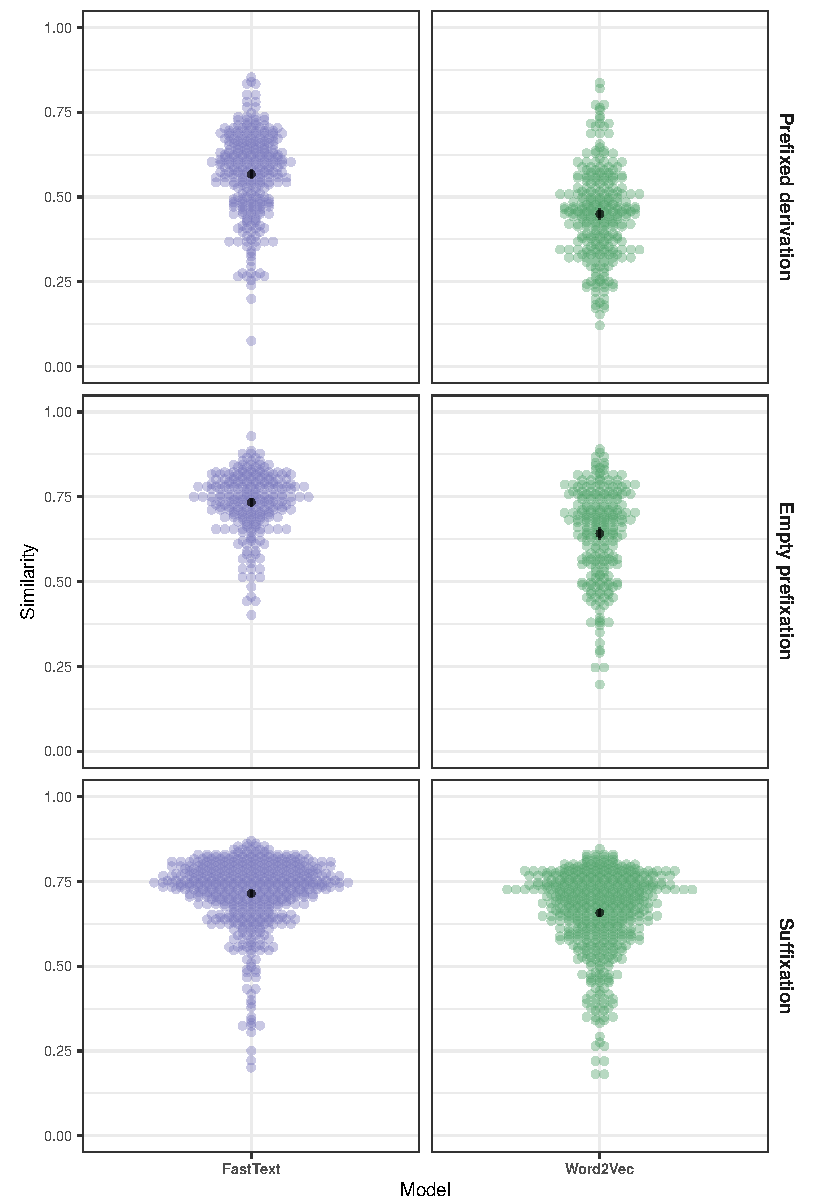
\includegraphics[height=16.5cm]{fig-aspect.pdf}
\caption{Similarity between an imperfective verb and three different ways of forming perfectives from it: prefixed derivation, empty prefixation and suffixation/stem alternation. Each coloured dot represents an imperfective-perfective pair. The black dot represents the mean similarity of all pairs.}
\label{fig:aspect}
\end{figure}


\begin{table}
    \centering
    \footnotesize
    \label{tbl:aspect-results}
    \begin{tabular}{lrrr}
        \toprule
        \textbf{Model} & \textbf{Derived} & \textbf{Empty prefix} & \textbf{Suffixed} \\
        \midrule
        \textbf{FastText} & 0.57 & 0.73 & 0.71 \\
        \textbf{Word2Vec} & 0.45 & 0.64 & 0.66 \\
        \bottomrule     
    \end{tabular}
    \caption{Mean similarity in Polish imperfective-perfective pairs.}
\end{table}

\subsection{Discussion} \label{discussion2}

% talk about the results and all, shortcomings?

Across both models, there is strong evidence that cosine similarity in forms with empty prefixes is comparable to that of inflectional suffixes, and both are markedly higher than the similarity observed in derivational prefixes. Regardless of whether the derivational forms are category-preserving, we find a consistent and substantial difference between inflectional and derivational morphology. These results suggest that empty prefixes pattern with inflectional morphology in terms of semantic similarity.

\section{General discussion} \label{gendiscussion}

This thesis has shed light on two different but related topics, the morphological inflection-derivation debate and the Polish aspectual marking debate. Using the methods developed in the first study, we tried to answer a theoretical question in the morphology of Polish.

How is it possible that we find contradictory evidence in the studies?

% The data and code used in this thesis can be found in a GitHub repository \footnote{https://github.com/gon-zalo/TFM-GLS}. The code is written in Python and uses different libraries located in the requirements.txt file.


\newpage
\addcontentsline{toc}{section}{References}
\sloppy
\printbibliography
\end{document}
